% ========================================
%	Header einbinden
% ========================================

\documentclass[bibtotoc,titlepage]{scrartcl}

% Deutsche Spracheinstellungen
\usepackage[ngerman,german]{babel, varioref}
\usepackage[T1]{fontenc}
\usepackage[utf8]{inputenc}

%\usepackage{marvosym}

\usepackage{amsfonts}
\usepackage{amssymb}
\usepackage{amsmath}
\usepackage{amscd}
\usepackage{amstext}

\usepackage{longtable}

%\usepackage{bibgerm}

\usepackage{footnpag}

\usepackage{ifthen}                 %%% package for conditionals in TeX
\usepackage[amssymb]{SIunits}
%Für textumflossene Bilder und Tablellen
%\usepackage{floatflt} - veraltet

%Für Testzwecke aktivieren, zeigt labels und refs im Text an.
%\usepackage{showkeys}

% Abstand zwischen zwei Absätzen nach DIN (1,5 Zeilen)
% \setlength{\parskip}{1.5ex plus0.5ex minus0.5ex}

% Einrückung am Anfang eines neuen Absatzes nach DIN (keine)
%\setlength{\parindent}{0pt}

% Ränder definieren
% \setlength{\oddsidemargin}{0.3cm}
% \setlength{\textwidth}{15.6cm}

% bessere Bildunterschriften
%\usepackage[center]{caption2}


% Problemlösungen beim Umgang mit Gleitumgebungen
\usepackage{float}

% Nummeriert bis zur Strukturstufe 3 (also <section>, <subsection> und <subsubsection>)
%\setcounter{secnumdepth}{3}

% Führt das Inhaltsverzeichnis bis zur Strukturstufe 3
%\setcounter{tocdepth}{3}
\usepackage[version=3]{mhchem}
	\mhchemoptions{minus-sidebearing-left=0.06em, minus-sidebearing-right=0.11em}
\usepackage{exscale}

\newenvironment{dsm} {\begin{displaymath}} {\end{displaymath}}
\newenvironment{vars} {\begin{center}\scriptsize} {\normalsize \end{center}}


\newcommand {\en} {\varepsilon_0}               % Epsilon-Null aus der Elektrodynamik
\newcommand {\lap} {\; \mathbf{\Delta}}         % Laplace-Operator
\newcommand {\R} { \mathbb{R} }                 % Menge der reellen Zahlen
\newcommand {\e} { \ \mathbf{e} }               % Eulersche Zahl
\renewcommand {\i} { \mathbf{i} }               % komplexe Zahl i
\newcommand {\N} { \mathbb{N} }                 % Menge der nat. Zahlen
\newcommand {\C} { \mathbb{C} }                 % Menge der kompl. Zahlen
\newcommand {\Z} { \mathbb{Z} }                 % Menge der kompl. Zahlen
\newcommand {\limi}[1]{\lim_{#1 \rightarrow \infty}} % Limes unendlich
\newcommand {\sumi}[1]{\sum_{#1=0}^\infty}
\newcommand {\rot} {\; \mathrm{rot} \,}         % Rotation
\newcommand {\grad} {\; \mathrm{grad} \,}       % Gradient
\newcommand {\dive} {\; \mathrm{div} \,}        % Divergenz
\newcommand {\dx} {\; \mathrm{d} }              % Differential d
\newcommand {\cotanh} {\; \mathrm{cotanh} \,}   %Cotangenshyperbolicus
\newcommand {\asinh} {\; \mathrm{areasinh} \,}  %Area-Sinus-Hyp.
\newcommand {\acosh} {\; \mathrm{areacosh} \,}  %Area-Cosinus-H.
\newcommand {\atanh} {\; \mathrm{areatanh} \,}  %Area Tangens-H.
\newcommand {\acoth} {\; \mathrm{areacoth} \,}  % Area-cotangens
\newcommand {\Sp} {\; \mathrm{Sp} \,}
\newcommand {\mbe} {\stackrel{\text{!}}{=}}     %Must Be Equal
\newcommand{\qed} { \hfill $\square$\\}
\renewcommand{\i} {\imath}
\def\captionsngerman{\def\figurename{\textbf{Abb.}}}

%%%%%%%%%%%%%%%%%%%%%%%%%%%%%%%%%%%%%%%%%%%%%%%%%%%%%%%%%%%%%%%%%%%%%%%%%%%%
% SWITCH FOR PDFLATEX or LATEX
%%%%%%%%%%%%%%%%%%%%%%%%%%%%%%%%%%%%%%%%%%%%%%%%%%%%%%%%%%%%%%%%%%%%%%%%%%%%
%%%
\ifx\pdfoutput\undefined %%%%%%%%%%%%%%%%%%%%%%%%%%%%%%%%%%%%%%%%% LATEX %%%
%%%
\usepackage[dvips]{graphicx}       %%% graphics for dvips
\DeclareGraphicsExtensions{.eps,.ps}   %%% standard extension for included graphics
\usepackage[ps2pdf]{thumbpdf}      %%% thumbnails for ps2pdf
\usepackage[ps2pdf,                %%% hyper-references for ps2pdf
bookmarks=true,%                   %%% generate bookmarks ...
bookmarksnumbered=true,%           %%% ... with numbers
hypertexnames=false,%              %%% needed for correct links to figures !!!
breaklinks=true,%                  %%% breaks lines, but links are very small
linkbordercolor={0 0 1},%          %%% blue frames around links
pdfborder={0 0 112.0}]{hyperref}%  %%% border-width of frames
%                                      will be multiplied with 0.009 by ps2pdf
%
\hypersetup{ pdfauthor   = {Hannes Franke; Julius Tilly},
pdftitle    = {V301 Innenwiderstand und Leistungsanpassung}, pdfsubject  = {Protokoll FP}, pdfkeywords = {V301, Innenwiderstand, Leistungsanpassung},
pdfcreator  = {LaTeX with hyperref package}, pdfproducer = {dvips
+ ps2pdf} }
%%%
\else %%%%%%%%%%%%%%%%%%%%%%%%%%%%%%%%%%%%%%%%%%%%%%%%%%%%%%%%%% PDFLATEX %%%
%%%
\usepackage[pdftex]{graphicx}      %%% graphics for pdfLaTeX
\DeclareGraphicsExtensions{.pdf}   %%% standard extension for included graphics
\usepackage[pdftex]{thumbpdf}      %%% thumbnails for pdflatex
\usepackage[pdftex,                %%% hyper-references for pdflatex
bookmarks=true,%                   %%% generate bookmarks ...
bookmarksnumbered=true,%           %%% ... with numbers
hypertexnames=false,%              %%% needed for correct links to figures !!!
breaklinks=true,%                  %%% break links if exceeding a single line
linkbordercolor={0 0 1},
linktocpage]{hyperref} %%% blue frames around links
%                                  %%% pdfborder={0 0 1} is the default
\hypersetup{
pdftitle    = {V301 Innenwiderstand und Leistungsanpassung}, 
pdfsubject  = {Protokoll AP}, 
pdfkeywords = {V301, Innenwiderstand, Leistungsanpassung},
pdfsubject  = {Protokoll AP},
pdfkeywords = {V301, Innenwiderstand, Leistungsanpassung}}
%                                  %%% pdfcreator, pdfproducer,
%                                      and CreationDate are automatically set
%                                      by pdflatex !!!
\pdfadjustspacing=1                %%% force LaTeX-like character spacing
\usepackage{epstopdf}
%
\fi %%%%%%%%%%%%%%%%%%%%%%%%%%%%%%%%%%%%%%%%%%%%%%%%%%% END OF CONDITION %%%
%%%%%%%%%%%%%%%%%%%%%%%%%%%%%%%%%%%%%%%%%%%%%%%%%%%%%%%%%%%%%%%%%%%%%%%%%%%%
% seitliche Tabellen und Abbildungen
%\usepackage{rotating}
\usepackage{ae}
\usepackage{
  array,
  booktabs,
  dcolumn
}
\makeatletter 
  \renewenvironment{figure}[1][] {% 
    \ifthenelse{\equal{#1}{}}{% 
      \@float{figure} 
    }{% 
      \@float{figure}[#1]% 
    }% 
    \centering 
  }{% 
    \end@float 
  } 
  \makeatother 


  \makeatletter 
  \renewenvironment{table}[1][] {% 
    \ifthenelse{\equal{#1}{}}{% 
      \@float{table} 
    }{% 
      \@float{table}[#1]% 
    }% 
    \centering 
  }{% 
    \end@float 
  } 
  \makeatother 
%\usepackage{listings}
%\lstloadlanguages{[Visual]Basic}
%\allowdisplaybreaks[1]
%\usepackage{hycap}
%\usepackage{fancyunits}


% ========================================
%	Angaben für das Titelblatt
% ========================================

\title{Versuch US1 - Grundlagen der Ultraschalltechnik\\				% Titel des Versuchs 
\large TU Dortmund, Fakultät Physik\\ 
\normalsize Anfänger-Praktikum}

\author{Jan Adam\\			% Name Praktikumspartner A
{\small \href{jan.adam@tu-dortmund.de}{jan.adam@tu-dortmund.de}}	% Erzeugt interaktiven einen Link
\and						% um einen weiteren Author hinzuzfügen
Dimitrios Skodras\\					% Name Praktikumspartner B
{\small \href{dimitrios.skodras@tu-dortmund.de}{dimitrios.skodras@tu-dortmund.de}}		% Erzeugt interaktiven einen Link
}
\date{23.Apirl 2013}				% Das Datum der Versuchsdurchführung

% ========================================
%	Das Dokument beginnt
% ========================================

\begin{document}

% ========================================
%	Titelblatt erzeugen
% ========================================

\maketitle					% Jetzt wird die Titelseite erzeugt
\thispagestyle{empty} 				% Weder Kopfzeile noch Fußzeile

% ========================================
%	Der Vorspann
% ========================================

%\newpage					% Wenn Verzeichnisse auf einer neuen Seite beginnen sollen
%\pagestyle{empty}				% Weder Kopf- noch Fußzeile für Verzeichnisse

\tableofcontents

%\newpage					% eine neue Seite
%\thispagestyle{empty}				% Weder Kopf- noch Fußzeile für Verzeichnisse
%\listoffigures					% Abbildungsverzeichnis

%\newpage					% eine neue Seite
%\thispagestyle{empty}				% Weder Kopf- noch Fußzeile für Verzeichnisse
%\listoftables					% Tabellenverzeichnis
\newpage					% eine neue Seite


% ========================================
%	Kapitel
% ========================================

%\section{Einleitung}				% Bei Bedarf

\section{Theorie}
Schall ist eine, sich auf Grund von Dichteschwankungen ausbreitende longditudinale Welle der Form:
\begin{formel}[H]
\center
	$p(x,t) = p_0 + v_0Zcos(wt-kx)$
	\caption*{\small{Z-akustische Impendanz}}
\end{formel}
Eine Schallwelle kann ebenso wie eine elektromagnetische Welle gebrochen und reflektiert werden, dagegen ist die Ausbreitungsgeschwindigkeit des Schall Materialabhängig:
\begin{align}
	c_{Flüssigkeit}&= \sqrt{\frac{1}{\kappa \cdot \rho}}\\
	c_{Festkörper}&= \sqrt{\frac{E}{\rho}}
\end{align}
Dabei ist $\kappa$ die Kompressibilität der Flüssigkeit und E das Elastizitätsmodul des Festkörpers.\\

Erzeugt werden kann Ultraschall auf verschiedene Arten. Im Experiment werden hierfür piezoellektrische Kristalle verwendet. Diese verändern unter dem Einfluss elektrischer Felder ihre Ausdehnung und können daher durch entsprechend schnelle Umpolung des Feldes zu einer Frequenz im Ultraschallbereich angeregt werden. Andersherum entsteht an den Enden eines solchen Kristalls eine Spannung, wenn Druck auf ihn ausgeübt wird. Daher kann mit dem Kristall auch Ultraschall gemessen werden.\\
Für die Untersuchung eines Körpers stehen verschiedene Messverfahren zur Auswahl:

\subsection{Durchschallungs-Verfahren}
Ultraschallsender und -Empfänger werden an gegenüberliegenden Seiten der Probe angebracht. Aus der zeitlichen Differenz zwischen aussenden eines Impulses und dem Auftreffen auf dem Empfänger kann man die Schallgeschwindigkeit im Medium bestimmen und daher Rücklüsse auf das Material ziehen.\\
Befindet sich eine Fehlstelle in der durchstrahlten Probe, so wird eine abgeschwächte Intensität am Ultraschallempfänger gemessen. Hierbei kann die Höhe der Differenz Aufschluß über die Größe der Fehlstelle geben. Eine
Aussage darüber, wo sich die Fehlstelle in der Probe befindet, ist jedoch nicht möglich.\\

\subsection{Impuls-Echo-Verfahren}
Beim Impuls-Echo-Verfahren wird der Ultraschallsender auch als Empfänger verwendet. Der ausgesendete Ultraschallpuls wird hierbei an einer Grenzfläche reflektiert und nach seiner Rückkehr von dem Empfänger aufgenommen. Bei bekannter Schallgeschwindigkeit kann aus der Laufzeit die Lage der Fehlstelle bestimmt werden, indem der durch die Fehlstelle auftretende Peak ausgewertet wird.\\
Die Schallwelle hat dabei in der Zeit $\Delta t$ folgende Strecke zurückgelegt
\begin{align}
	\Delta s = \frac{1}{2} c \cdot \Delta t
	\label{eq_strecke}
\end{align}

\subsection{A- und B-Scan}
Die Messwerte aus den Sonden können auf verschiedene Arten dargestellt werden:\\

Der Amplituden Scan ist ein eindimensionales Verfahren und stellt jeden Aufgenommenen Impuls als einen Peak auf der Zeitachse mit einer Höhe, die der Intensität entspricht.\\

Der Brightness Scan erzeugt durch bewegen der Sonde ein zweidimensionals Bild dar. Die Amplitudenstärke wird durch Helligkeitsabstufungen oder verschieden Farbtöne dargestellt.


\section{Durchführung}
Im Versuch sollen die Schallgeschwindigkeit in einem Acryllblock sowie die Lage und Größe verschiedener Fehlstellen in selbigem bestimmt werden. 
\begin{wrapfigure}[6]{r}{3.5cm}
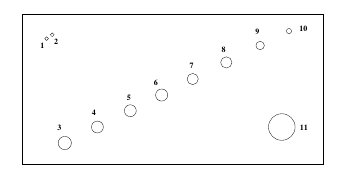
\includegraphics[width=0.2\textwidth]{pics/block.jpg}
\caption{\mbox{Acryllblock}}
\end{wrapfigure}
Anschließend soll mittels A-Scan die Abmessung eines Augemodells berechnet werden.

\begin{wrapfigure}[6]{r}{3.5cm}
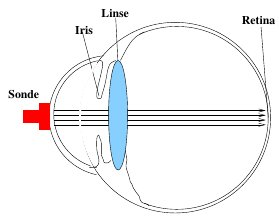
\includegraphics[width=0.2\textwidth]{pics/auge.jpg}
\caption{\mbox{Augenmodell}}
\end{wrapfigure}

Zunächst werden verschieden lange Acryllzylinder mittels Durchlaufverfahren beschallt. Aus der Laufzeit der Welle und der bekannten Abmessung des Zylinders wird so die Schallgeschwindigkeit im Acryll bestimmt.

Anschließend wird der Acryllblock mit den Fehlstellen untersucht. Hierzu verwendet man das Echo-Impuls-Verfahren auf beiden Seiten des Blockes um die genaue Lage und die Ausdehnung der Löcher zu finden.

Das Augenmodell wird ebenfalls mit dem Echo-Impulsverfahren untersucht. Gemessen werden sollen die Abstände: Hornhaut-Iris, -Linse und -Retina.


\section{Auswertung}
\subsection{Fehlerrechnung}
Da viele für die Auswertung notwendigen Größen fehlerbehaftet sind, ist es wichtig, den Einfluss dieser Fehler auf die ermittelten
Größen herauszufinden. Neben den, von den Messapparaturen verursachten Fehlern, dienen der Mittelwert
\begin{formel}[H]
\begin{equation}
 \bar{x} = \frac1N \sum_{i=1}^{N} x_i,
 \label{eq_mittel}
\end{equation}
\caption*{\small{$\bar{x}$ = Mittelwert, N = Anzahl der Messungen}}
\end{formel}

die Gaußsche Fehlerfortpflanzung

\begin{formel}[H]
\begin{equation}
\Delta G = \sqrt{\sum_{i=1}^{N}\left( \frac{\partial G}{\partial x_i}\cdot \Delta x_i\right)^2},
\label{gauss}
\end{equation}
\caption*{$x_i$ = Variable, $\Delta x_i$ = Fehler der Variable}
\end{formel}
und die Standardabweichung des Mittelwerts

\begin{equation}
 \bar s = \sqrt{\frac{1}{N(N-1)} \sum_{i}^{N} (x_i - \bar{x})^2}.
 \label{eq_standard}
\end{equation}

\subsection{Schallgeschwidigkeit in Acryl}
Um in Abschnitt \ref{sec_bohrung} die Abmessungen der Bohrungen in einem Acrylblock ermitteln zu können, ist die Bestimmung der Schallgeschwidigkeit 
in Acryl vonnöten. Hierzu werden das Impuls-Echo-Verfahren und das Durchschallungs-Verfahren genutzt. Zuvor werden die Höhen der verwandten
Acrylzylinder, sowie des -blocks mit einer Schieblehre ausgemessen, nach \eqref{eq_mittel} gemittelt und ihr Fehler entsprechend 
\eqref{eq_standard} bestimmt. Die Ergebnisse sind in Tabelle \ref{tab_masse} aufgeführt.

\begin{table}[H]
 \begin{tabular}{c|c|c|c|c}
  & Klein & Mittel & Groß & Block\\
  \hline
	&39,6&	80,5&	120,7&	77,3\\
Höhe 	&39,7&	80,4&	120,7&	77,6\\
in 	&39,7&	80,5&	120,6&	77,5\\
mm 	&39,7&	80,5&	120,5&	77,6\\
	&39,7&	80,5&	120,5&	77,7\\
	\hline
Mittelwert	&39,68$\pm$0,0004&	80,48$\pm$0,0004 &	120,6$\pm$0,002&	77,54$\pm$0,0046
 \end{tabular}
 \caption{Ausmaße verwandter Acrylkörper}
\label{tab_masse}
\end{table}

\subsubsection{Bestimmung mittels Impuls-Echo-Verfahren}
In Tabelle \ref{tab_impulsecho} ist für die drei Zylinder die durch drei verschiedene Ultrschallsonden gemessene Laufzeit aufgeführt. Der
entstehende Fehler von $\Delta t$ = 0,1 $\mu$s wird vom Computerprogramm angegeben.

\begin{table}[H]
 \begin{tabular}{c|c|c|c}
 Ultraschallsonde & Klein & Mittel & Groß\\
 \hline
1 MHz (blau)&	30,6&	60,4&	89,7\\
2 MHz (rot)&	29,9&	59,7&	88,8\\
4 MHz (grün)&	29,4&	59,1&	88,5\\  
 \end{tabular}
\caption{Laufzeiten in $\mu$s bei den Acrylkörpern mit drei Sonden}
\label{tab_impulsecho}
\end{table}

Aufgrund der Anpassungsschicht der Ultrschallsonden, muss die Gleichung \eqref{eq_fehlstelle} um den Laufzeitfehler $t_f$ modifiziert werden.
Aus der Differenz der Laufzeitstrecken $\delta s$ in \eqref{eq_laufzeitstrecke} lässt sich die Schallgeschwidigkeit in Acryl ohne 
Laufzeitfehler bestimmen. Die Gleichungen

\begin{align}
\label{eq_laufzeitfehler}
 s_i &= \frac12 c (t_i - t_f)\\
 \nonumber
 s_j &= \frac12 c (t_j - t_f)\\
 \delta s &= s_i - s_j = \frac12 c \cdot  \delta t = \frac12 c (t_i - t_j)
 \label{eq_laufzeitstrecke}
\end{align}
führen zur Schallgeschwidigkeit

\begin{align}
 c = 2\, \frac{\delta s}{\delta t}.
\end{align}
Ihr Fehler errechnet sich aus \eqref{gauss} zu

\begin{align}
 \Delta c = \sqrt{\left(\frac{\partial c}{\partial \delta s} \Delta s \right)^2 + \left(\frac{\partial c}{\partial \delta t} \Delta t \right)^2} = c\, \sqrt{\frac{\Delta s}{\delta s}^2 + \frac{\Delta t}{\delta t}^2}.
\end{align}
In Tabelle \ref{tab_schall} sind die Ergebnisse zur Schallgeschwidigkeit aufgeführt. 
\renewcommand{\arraystretch}{1.5}
\begin{table}[H]
 \begin{tabular}{c|c|c|c|c}
Sonde & Größe & Klein-Groß & Klein-Mittel & Mittel-Groß\\
\hline
&$\delta s$ in mm	&	80,92$\pm$0,002&	40,80$\pm$0,0005&	40,12$\pm$0,002\\
\hline
\hline
1 MHz &$\delta t$ in $\mu$s &59,1$\pm$0,1&	29,8$\pm$0,1&	29,3$\pm$0,1\\
&$c$ in km/s		&2,74$\pm$0,0046&	2,74$\pm$0,0092	&	2,74$\pm$,0093\\
\hline
2 MHz &$\delta t$ in $\mu$s &	58,9$\pm$0,1&	29,8$\pm$0,1&	29,1$\pm$0,1\\
&$c$ in km/s		&2,75$\pm$0,0047&	2,74$\pm$0,0092	&	2,76$\pm$,0095\\
\hline
4 MHz &$\delta t$ in $\mu$s &	59,1$\pm$0,1&	29,7$\pm$0,1&	29,4$\pm$0,1\\
&$c$ in km/s		&2,74$\pm$0,0046&	2,75$\pm$0,0093&	2,73$\pm$,0093\\
 \end{tabular}
\caption{Schallgeschwidigkeit $c$ in Acryl}
\label{tab_schall}
\end{table}
\renewcommand{\arraystretch}{1.0}
Aus den Werten ergibt sich für die Schallgeschwidigkeit in Acryl ein gemittelter Wert von

\begin{align}
 c = 2,742\pm0,003 \text{km/s}.
\end{align}

Der in Abschnitt \ref{sec_bohrung} benutzte Acrylblock wird mit der blauen Ultraschallsonde untersucht. Der dort ebenfalls auftretende
Laufzeitfehler $t_f$ kann mit der ermittelten Schallgeschwidigkeit nach \eqref{eq_laufzeitfehler} errechnet werden. Das Ergebnis
ist in Tabelle \ref{tab_laufzeitfehler} zu finden.

\begin{table}[H]
 \begin{tabular}{c|c|c|c|c}
Blaue Sonde & Klein & Mittel & Groß & Mittelwert\\
 \hline
  $t_f$ in $\mu$s &1,65$\pm$	&1,69$\pm$	&1,72$\pm$ & 1,69$\pm$ \\
 \end{tabular}

\end{table}



\subsubsection{Bestimmung mittels Durchschallungs-Verfahren}
\subsection{Untersuchung von Bohrungen in einem Acrylblock}
\label{sec_bohrung}
\subsection{Biometrische Untersuchung eines Augenmodells}

\section{Diskussion}

% ========================================
%	Literaturverzeichnis
% ========================================

%\bibliographystyle{plainnat}			% Bibliographie-Style auswählen
%\bibliography{BIBDATEI}			% Literaturverzeichnis

% ========================================
%	Das Dokument endent
% ========================================

\end{document}
